\chapter{S\`{e}ries de Fourier}\label{sec:serie_fu} \index{s\`{e}ries de
Fourier}

\section{Definicions}\index{s\`{e}ries de Fourier!definicions}

Una funci\'{o} peri\`{o}dica en el temps $v(t)$, de freq\"{u}\`{e}ncia $f$, per\'{\i}ode
$T$ i velocitat angular $\omega$ ($f = 1/T$, $\omega=2\piup f =
2\piup\,/T$), es pot expressar com una suma infinita de funcions sinus i
cosinus; \'{e}s el que s'anomena expansi\'{o} d'una funci\'{o} peri\`{o}dica en
s\`{e}rie de Fourier:
\begin{equation}
    v(t) = A_0 + \sum_{n=1}^\infty A_n \cos (n \omega t) +
    \sum_{n=1}^\infty B_n \sin (n \omega t) \label{eq:serie_fu_wt}
\end{equation}

Els coeficients $A_0$, $A_n$ i $B_n$, es calculen a partir de les
expressions seg\"{u}ents:
\begin{subequations}
\begin{alignat}{3}
    A_0 &= \frac{1}{T} \int_{t_0}^{t_0+T}\!  v(t) \diff t &&=
    \frac{\omega}{2\piup} \int_{t_0}^{t_0+\frac{2\piup} {\omega}} \! v(t) \diff
    t \label{eq:a0_t} & \\[0.5ex]
    A_n &= \frac{2}{T} \int_{t_0}^{t_0+T}\!  v(t) \cos(n \omega t) \diff
    t &&=
    \frac{\omega}{\piup} \int_{t_0}^{t_0+\frac{2\piup}{\omega}} \! v(t)\cos(n \omega t) \diff
    t &\qquad(n=1,\ldots\infty)\\[0.5ex]
    B_n &= \frac{2}{T} \int_{t_0}^{t_0+T}\!  v(t) \sin(n \omega t) \diff t
    &&=
    \frac{\omega}{\piup} \int_{t_0}^{t_0+\frac{2\piup}{\omega}}\!  v(t)\sin(n \omega t) \diff
    t &\qquad(n=1,\ldots\infty)
\end{alignat}
\end{subequations}

Si la funci\'{o} peri\`{o}dica $v(\alpha)$ est\`{a} definida en funci\'{o} de
l'angle $\alpha$, enlloc del temps $t$, a partir de la relaci\'{o}
$\alpha=\omega t$ ($\diff\alpha=\omega\diff t$), tenim:
\begin{equation}
    v(\alpha) = A_0 + \sum_{n=1}^\infty A_n \cos n \alpha +
    \sum_{n=1}^\infty B_n \sin n \alpha \label{eq:serie_fu_alfa}
\end{equation}

En aquest cas, els coeficients $A_0$, $A_n$ i $B_n$, es calculen a
partir de les expressions seg\"{u}ents:
\begin{subequations}
\begin{alignat}{2}
    A_0 &= \frac{1}{2\piup} \int_{\alpha_0}^{\alpha_0+2\piup} \! v(\alpha) \diff \alpha
    \label{eq:a0_alfa} & \\[0.5ex]
    A_n &= \frac{1}{\piup} \int_{\alpha_0}^{\alpha_0+2\piup} \! v(\alpha) \cos n \alpha \diff
    \alpha &\qquad(n=1,\ldots\infty)\\[0.5ex]
    B_n &= \frac{1}{\piup} \int_{\alpha_0}^{\alpha_0+2\piup} \! v(\alpha) \sin n \alpha \diff \alpha
    &\qquad(n=1,\ldots\infty)
\end{alignat}
\end{subequations}

Les equacions \eqref{eq:serie_fu_wt} i \eqref{eq:serie_fu_alfa} es
poden expressar d'una manera alternativa, utilitzant \'{u}nicament
funcions cosinus, quan $v(t)$ \'{e}s una funci\'{o} real i per tant $A_n, B_n \in \mathbb{R}$:
\begin{align}
    v(t) &= C_0 + \sum_{n=1}^\infty C_n \cos (n \omega t + \phi_n)
    \label{eq:serie_f_c_t}\\[0.5ex]
    v(\alpha) &= C_0 + \sum_{n=1}^\infty C_n \cos (n \alpha +
    \phi_n)\label{eq:serie_f_c_alfa}
\end{align}

Els coeficients $C_0$, $C_n$ i $\phi_n$\footnote{Cal tenir en compte que la funci\'{o} \textsf{arctan} disponible en moltes calculadores i llenguatges de programaci\'{o}, torna de forma estandarditzada valors compresos entre $-\frac{\piup}{2}$ i $\frac{\piup}{2}$. En aquest cas cal sumar el valor $\piup$, quan $A_n$ \'{e}s negatiu, a l'angle obtingut amb la funci\'{o} \textsf{arctan} per tal d'obtenir l'angle en el quadrant correcte.}, amb $A_n,B_n\in\mathbb{R}$, es calculen a partir de les
expressions seg\"{u}ents:
\begin{subequations}
\begin{alignat}{2}
    C_0 &= A_0 & \\[0.5ex]
    C_n &= \sqrt{A_n^2+B_n^2} &\qquad(n=1,\ldots\infty)\\[0.5ex]
    \phi_n &= \begin{cases} -\arctan \dfrac{B_n}{A_n}, & A_n\neq0\\[1.5ex]
    -\dfrac{\pi}{2}, & A_n=0\end{cases}
     &\qquad(n=1,\ldots\infty)\label{eq:serie_f_fi}
\end{alignat}
\end{subequations}


Si comparem l'equaci\'{o} \eqref{eq:a0_t} amb l'equaci\'{o} \eqref{eq:vm_t}
o l'equaci\'{o} \eqref{eq:a0_alfa} amb l'equaci\'{o} \eqref{eq:vm_alfa},
veurem que s\'{o}n id\`{e}ntiques, i per tant es pot afirmar que el
coeficient $A_0$ (i per tant, tamb\'{e} $C_0$) \'{e}s igual al valor mitj\`{a} de la
funci\'{o} peri\`{o}dica.

Atenent a les equacions  \eqref{eq:serie_f_c_t} o
\eqref{eq:serie_f_c_alfa}, el terme d'\'{\i}ndex $n=1$, $C_1 \cos (\omega
t + \phi_1)$ o $C_1 \cos (\alpha + \phi_1)$,  s'anomena component
fonamental, perqu\`{e} t\'{e} la mateixa freq\"{u}\`{e}ncia que la funci\'{o} original.
La resta de termes, d'\'{\i}ndex $n=2,\ldots,\infty$, s'anomenen
components harm\`{o}niques.

\section{Simplificacions}\index{s\`{e}ries de Fourier!simplificacions}

Quan les funcions $v(t)$ o $v(\alpha)$ presenten certes simetries,
alguns dels coeficients $A_n$, $B_n$, $C_n$ i $\phi_n$ s'anu{\l.l}en, o
prenen valors determinats.

\subsection{Funcions parells}\index{funci\'{o}!parell}

S\'{o}n funcions que compleixen: $v(t) = v(-t)$ o $v(\alpha) =
v(-\alpha)$. En aquest cas,  tots els coeficients $B_n$ s'anu{\l.l}en;
en concret tenim:
\begin{subequations}
\begin{alignat}{2}
    B_n &= 0       &\qquad (n = 1,\ldots,\infty)\\[0.5ex]
    C_0 &= A_0 \\[0.5ex]
    C_n &= A_n     &\qquad (n = 1,\ldots,\infty)\\[0.5ex]
    \phi_n &= 0 &\qquad (n = 1,\ldots,\infty)
\end{alignat}
\end{subequations}


\break
\subsection{Funcions senars}\index{funci\'{o}!senar}

S\'{o}n funcions que compleixen: $v(t) = -v(-t)$ o $v(\alpha) =
-v(-\alpha)$. En aquest cas,  tots els coeficients $A_n$ s'anu{\l.l}en;
en concret tenim:
\begin{subequations}
\begin{alignat}{2}
    A_0 &= 0       & \\[0.5ex]
    A_n &= 0       &\qquad (n = 1,\ldots,\infty)\\[0.5ex]
    C_0 &= 0    \\[0.5ex]
    C_n &= B_n     &\qquad (n = 1,\ldots,\infty)\\[0.5ex]
    \phi_n &= -\frac{\piup}{2} &\qquad (n = 1,\ldots,\infty)
\end{alignat}
\end{subequations}

\subsection{Funcions amb simetria de semiona}\index{funci\'{o}!amb simetria de semiona}

S\'{o}n funcions que compleixen: $v(t) = -v(t+\frac{T}{2})$ o $v(\alpha) = -v(\alpha+\piup)$. En aquest
cas, tots els coeficients $A_n$ i $B_n$ d'\'{\i}ndex parell s'anu{\l.l}en;
en concret tenim:
\begin{subequations}
\begin{alignat}{2}
    A_0 &= 0       & \\[0.5ex]
    A_n &= 0       &\qquad (n = 2,4,6,\ldots,\infty)\\[0.5ex]
    B_n &= 0       &\qquad (n = 2,4,6,\ldots,\infty)\\[0.5ex]
    C_n &= 0       &\qquad (n = 2,4,6,\ldots,\infty)\\[0.5ex]
    \phi_n &= 0 &\qquad (n = 2,4,6,\ldots,\infty)
\end{alignat}
\end{subequations}

\section{Condici\'{o} de Dirichlet}\index{Dirichlet, condici\'{o} de}
\index{s\`{e}ries de Fourier!condici\'{o} de Dirichlet}

Quan una funci\'{o} peri\`{o}dica $v(t)$  \'{e}s cont\'{\i}nua en tot el seu per\'{\i}ode
$T$, la seva expansi\'{o} en s\`{e}rie de Fourier convergeix al mateix valor
que la funci\'{o} original, per a qualsevol valor de $t$.

En el cas que la funci\'{o} $v(t)$ estigui definida a trossos, com per
exemple una ona quadrada, la condici\'{o} de Dirichlet ens assegura que
la seva expansi\'{o} en s\`{e}rie de Fourier convergeix al mateix valor que
la funci\'{o} original, per a tots els valors de $t$ on la funci\'{o} es
cont\'{\i}nua, i que en els punts de discontinu\"{\i}tat de la funci\'{o}, la seva
expansi\'{o} en s\`{e}rie de Fourier convergeix al valor mitj\`{a} dels l\'{\i}mits
per la dreta i per l'esquerra de la funci\'{o} en aquests punts. Per tal
que aix\`{o} es compleixi, la funci\'{o} $v(t)$ ha de complir les condicions
seg\"{u}ents:
\begin{dinglist}{'167}
   \item Ha de tenir un nombre finit de discontinu\"{\i}tats
   finites.
   \item Ha de tenir un nombre finit d'extrems (m\`{a}xims o m\'{\i}nims).
\end{dinglist}

Tot el que s'ha dit \'{e}s igualment v\`{a}lid per a una funci\'{o} peri\`{o}dica
$v(\alpha)$  definida en funci\'{o} de l'angle $\alpha$.


\section{Valors mitj\`{a} i efica\c{c}, taxes, factors i distorsi\'{o} harm\`{o}nica total}\label{sec:four_val_mitja_ef}

\subsection{Valor mitj\`{a}}\label{sec:four_val_av}
\index{valor!mitj\`{a}}
\index{s\`{e}ries de Fourier!valor mitj\`{a}}

Com ja s'ha dir anteriorment, el valor mitj\`{a} $\bar{V}$ d'una
funci\'{o} peri\`{o}dica $v(t)$ o $v(\alpha)$ \'{e}s:
\begin{equation}
    \bar{V} = A_0 = C_0
\end{equation}

\subsection{Valor efica\c{c}}\label{sec:four_val_ef}
\index{valor!efica\c{c}}\index{s\`{e}ries de Fourier!valor efica\c{c}}

Atenent a les equacions  \eqref{eq:serie_f_c_t} o
\eqref{eq:serie_f_c_alfa}, els valors de cresta $\hat{V}_n$ i efica\c{c}
$V_n$ de cadascun dels termes del sumatori, s\'{o}n respectivament
\begin{alignat}{2}
    \hat{V}_n &= C_n &\qquad(n=1,\ldots,\infty)\\[0.5ex]
    V_n &= \frac{C_n}{\sqrt{2}} &\qquad(n=1,\ldots,\infty)
\end{alignat}

El valor efica\c{c} total $V$ de  la funci\'{o} peri\`{o}dica $v(t)$ o
$v(\alpha)$ \'{e}s:
\begin{equation}
    V = \sqrt{\bar{V}^2 + \sum_{n=1}^{\infty}V^2_n} \label{eq:val_ef_fourier}
\end{equation}

\subsection{Taxa de fonamental}
\index{g@$g$}\index{taxa!de  fonamental}\index{s\`{e}ries de Fourier!taxa de fonamental}
La taxa  de fonamental relaciona el valor efica\c{c} de la component fonamental $V_1$, amb el valor efica\c{c}
total $V$. La norma \textsf{CEI 60050} l'anomena {"<}fundamental factor{">} o {"<}relative fundamental content{">}, li assigna el s\'{\i}mbol $g$ i la defineix com:\index{CEI!60050-00@60050}
\begin{equation}
    g = \frac{V_1}{V}
\end{equation}

Un valor proper a 1 indica  que les components harm\`{o}niques tenen poca import\`{a}ncia:

\subsection{Taxa de l'harm\`{o}nica d'ordre n}
\index{taxa!de l'harm\`{o}nica d'ordre n}\index{g@$g_n$}\index{s\`{e}ries de Fourier!taxa de l'harm\`{o}nica d'ordre n}

La taxa de l'harm\`{o}nica d'ordre $n$  relaciona el valor efica\c{c} d'aquesta harm\`{o}nica  $V_n$, amb el valor efica\c{c} de la component fonamental
 $V_1$. La norma \textsf{CEI 60050} l'anomena {"<}nth harmonic ratio{">} i la defineix com:\index{CEI!60050-00@60050}
\begin{equation}
    \frac{V_n}{V_1}
\end{equation}


\subsection{Taxa d'harm\`{o}niques}
\index{taxa!d'harm\`{o}niques}\index{d@$d$} \index{s\`{e}ries de Fourier!taxa d'harm\`{o}niques}

La taxa d'harm\`{o}niques relaciona el valor efica\c{c}  que
s'obtindria sense tenir en compte  la component fonamental $V_1$, amb el valor
efica\c{c} total $V$. La norma \textsf{CEI 60050} l'anomena {"<}total harmonic factor{">}, li assigna el s\'{\i}mbol $d$ i la defineix com:\index{CEI!60050-00@60050}
\begin{equation}
    d = \frac{\sqrt{\bar{V}^2+\displaystyle\sum_{n=2}^\infty V^2_n}}{V}
\end{equation}

Quan el valor mitj\`{a} $\bar{V}$ \'{e}s nul, es verifica:
\begin{equation}
    \bar{V}=0 \quad \Rightarrow\quad g^2 = 1 - d^2
\end{equation}

Un valor proper a 0 indica un baix contingut de components harm\`{o}niques.

\subsection{Distorsi\'{o} harm\`{o}nica total} \index{distorsi\'{o} harm\`{o}nica
total}\index{THD}\index{s\`{e}ries de Fourier!distorsi\'{o} harm\`{o}nica total}

 La distorsi\'{o} harm\`{o}nica total  relaciona el valor efica\c{c}  que
s'obtindria sense tenir en compte  la component fonamental $V_1$,
amb el valor efica\c{c} d'aquesta component fonamental. La norma \textsf{CEI 60050} l'anomena {"<}total harmonic distortion (THD){">} i la defineix com:\index{CEI!60050-00@60050}
\begin{equation}
    \text{THD} = \frac{\sqrt{\bar{V}^2+  \displaystyle\sum_{n=2}^\infty V^2_n}} {V_1}
\end{equation}

Quan el valor mitj\`{a} $\bar{V}$ \'{e}s nul, es verifica:
\begin{equation}
   \bar{V}=0 \quad \Rightarrow\quad g^2 = \frac{1}{1+\text{THD}^2}
\end{equation}

Un valor proper a 0 indica un baix contingut de components harm\`{o}niques.

\subsection{Factor d'arrissada efica\c{c}}\label{sec:four_fac_arr_ef}
\index{factor!d'arrissada efica\c{c}}\index{r@$r$}\index{s\`{e}ries de Fourier!factor d'arrissada efica\c{c}}

El factor d'arrissada efica\c{c} relaciona el valor efica\c{c}  que
s'obtindria sense tenir en compte el valor mitj\`{a}  $\bar{V}$, amb aquest
valor mitj\`{a}. La norma \textsf{CEI 60050} l'anomena {"<}rms-ripple factor{">} o {"<}relative ripple content{">}, li assigna el s\'{\i}mbol $r$ i el defineix com:\index{CEI!60050-00@60050}
\begin{equation}
    r = \frac{\sqrt{\displaystyle\sum_{n=1}^\infty V^2_n}}{|\bar{V}|}
\end{equation}

Aquesta relaci\'{o} \'{e}s la mateixa que es pot veure en l'equaci\'{o}  \eqref{eq:rms_rip}, nom\'{e}s cal substituir-hi el valor efica\c{c} $V$ pel valor donat en l'equaci\'{o} \eqref{eq:val_ef_fourier}.

\subsection{Factor d'arrissada}\index{factor!d'arrissada}\index{r@$s$}\index{s\`{e}ries de Fourier!factor d'arrissada}

El factor d'arrissada relaciona el valor efica\c{c}  que
s'obtindria sense tenir en compte el valor mitj\`{a}  $\bar{V}$, amb el
valor efica\c{c} total $V$. La norma \textsf{CEI 60050} l'anomena {"<}pulsating factor{">}, li assigna el s\'{\i}mbol $s$ i el defineix com:\index{CEI!60050-00@60050}
\begin{equation}
    s = \frac{\sqrt{\displaystyle\sum_{n=1}^\infty V^2_n}}{V}
\end{equation}


\begin{exemple}[C\`{a}lcul de valors mitj\`{a} i efica\c{c} i de taxa de fonamental]
    Es tracta de calcular els valors mitj\`{a} i efica\c{c} i la taxa de
    fonamental, de la tensi\'{o} que s'obt\'{e} a partir d'una tensi\'{o}
    sinuso\"{\i}dal $u(t) = \hat{U} \sin\omega t$, amb un rectificador d'ona
    completa, utilitzant la seva expansi\'{o} en s\`{e}rie de Fourier.

    La tensi\'{o} que s'obt\'{e} del rectificador d'ona completa ve definida
    per:

    \[
    u(t) = \begin{cases} \phantom{-}\hat{U} \sin\omega t, & 0 < \omega t < \piup\\
           -\hat{U} \sin\omega t, & \piup \leq \omega t \leq 2\piup \end{cases}
    \]

    En aquest cas, l'ona de tensi\'{o} entre $\piup$ i $2\piup$ \'{e}s una repetici\'{o}
    exacta de l'ona de tensi\'{o} entre 0 i $\piup$, per tant, \'{u}nicament
    caldr\`{a} considerar-ne la primera meitat (entre 0 i $\piup$), tenint en
    compte que el per\'{\i}ode ser\`{a} $\piup\,/\omega$. A m\'{e}s, aquesta funci\'{o} \'{e}s
    parell $u(t) = u(-t)$, i per tant, tots els termes
    $B_n\;(n=1,\ldots,\infty)$ seran nuls.

    El terme $A_0$ val:

    \[
    A_0 = \frac{\omega}{\piup} \int_0^{\frac{\piup}{\omega}} \hat{U} \sin
    \omega t \diff t = \left. -\frac{\hat{U} \cos \omega t}{\piup}
    \right|_0^{\frac{\piup}{\omega}} = \frac{2\hat{U}}{\piup}
    \]

    Els temes $A_n$ valen:

    \[
    \begin{split}
    A_n &= \frac{2 \omega}{\piup} \int_0^{\frac{\piup}{\omega}} \hat{U} \sin
    \omega t \cos(n \omega t)\diff t = \left. \frac{2 \hat{U}[ \cos
    \omega t \cos (n \omega t) + n \sin \omega t \sin(n \omega
    t)]}{\piup(n^2-1)} \right|_0^{\frac{\piup}{\omega}}=\\[0.5ex]
    &= -\frac{2\hat{U}(1+\cos n \piup)}{\piup(n^2-1)}
    \qquad(n=1,\ldots,\infty)
    \end{split}
    \]

    Per tant, la funci\'{o} peri\`{o}dica $u(t)$ es pot expressar com:

    \[
        u(t) = \frac{2\hat{U}}{\piup} - \sum_{n=1}^\infty
         \frac{2\hat{U}(1+\cos n \piup)}{\piup(n^2-1)} \cos(n \omega t)
    \]

    Ara b\'{e}, si ens fixem en els termes $1+\cos n \piup$, veiem que valen 0
    per a $n=1,3,5,\ldots$ i 2 per a $n=2,4,6,\ldots$, i per tant, dins
    del sumatori \'{u}nicament ens quedaran termes d'\'{\i}ndex parell. Si a
    continuaci\'{o}, fem el canvi de variable $n=2k\;(n^2=4k^2)$, tenim:

    \[
    u(t) = \frac{2\hat{U}}{\piup} - \frac{4\hat{U}}{\piup} \sum_{k=1}^\infty
          \frac{\cos(2 k \omega t)}{4k^2-1}
    \]

    Aquesta simplificaci\'{o} es deguda al fet que s'ha utilitzat com a
    per\'{\i}ode de la funci\'{o} $u(t)$ la meitat $(\piup\,/\omega)$ del valor total
    $(2\piup\,/\omega)$, i per tant, \'{e}s com si n'hagu\'{e}ssim doblat la
    freq\"{u}\`{e}ncia i la velocitat angular; aix\'{\i} doncs, la velocitat angular
    de la component fonamental \'{e}s $2\omega$, i la velocitat angular de
    les components harm\`{o}niques \'{e}s $2\omega k \;(k=2,3,4,5\ldots)$.

    El valor mitj\`{a} $\bar{U}$ de $u(t)$ \'{e}s directament:

    \[
        \bar{U} = \frac{2\hat{U}}{\piup}
    \]

    El valor efica\c{c} de cadascun dels termes del sumatori \'{e}s:
    \[
        U_k =\frac{4\hat{U}}{\sqrt{2}\piup(4k^2-1)}
        \qquad(k=1,\ldots,\infty)
    \]

    El valor efica\c{c} total \'{e}s, per tant:

    \[
        U=\sqrt{\left(\frac{2\hat{U}}{\piup}\right)^2 + \sum_{k=1}^\infty
        \left(\frac{4\hat{U}}{\sqrt{2}\piup(4k^2-1)}\right)^2} =
        \sqrt{\frac{4\hat{U}^2}{\piup^2} + \frac{(\piup^2-8)\hat{U}^2}{2\piup^2}
        }= \frac{\hat{U}}{\sqrt{2}}
    \]

    Com es pot veure, aquests valors mitj\`{a} i efica\c{c} obtinguts aqu\'{\i}, s\'{o}n
    id\`{e}ntics als obtinguts en l'exemple de la Secci\'{o}
    \ref{sec:val_mitja_ef}.

    El valor efica\c{c} $U_1$ de la component fonamental val:

    \[
        U_1 =\frac{4\hat{U}}{\sqrt{2}\piup(4\times 1^2-1)} =
        \frac{4\hat{U}}{3\sqrt{2}\piup}
    \]

    La taxa de fonamental val, per tant:

    \[
        g =
        \frac{\dfrac{4\hat{U}}{3\sqrt{2}\piup}}{\dfrac{\hat{U}}{\sqrt{2}}}
        =\frac{4}{3\piup} = 0,{42}
    \]

    Com es pot veure, aquest valor no es gaire alt, aix\`{o} ens indica que
    el contingut de components harm\`{o}niques de la tensi\'{o} $u(t)$ \'{e}s
    elevat.
\end{exemple}


\section{Taula de s\`{e}ries de Fourier}\index{s\`{e}ries de Fourier!taula}

Encara que els coeficients de la s\`{e}rie de Fourier d'una funci\'{o} qualsevol es poden
obtenir resolent les integrals referides en les seccions anteriors, els c\`{a}lculs
involucrats poden ser for\c{c}a complicats; per aquest motiu, \'{e}s usual
disposar de taules que recullen les s\`{e}ries de Fourier d'un
gran nombre de funcions.

En la Taula \vref{taula:Serie-Fourier-Graf}, es pot veure una relaci\'{o} de
s\`{e}ries de Fourier de diverses formes d'ona usuals. Com \'{e}s habitual tenim: $\omega=2\piup f = 2\piup\, / T$.

\begin{longtable}{cc}
   \caption{\label{taula:Serie-Fourier-Graf} S\`{e}ries de Fourier de formes d'ona}\\
   \toprule[1pt]
   $f(t)$ & s\`{e}rie de Fourier de $f(t)$\\
   \midrule
   \endfirsthead
   \caption[]{S\`{e}ries de Fourier de formes d'ona (\emph{ve de la p\`{a}gina anterior})} \\
   \toprule[1pt]
   $f(t)$ & s\`{e}rie de Fourier de $f(t)$\\
   \midrule
   \endhead
   \midrule
   \multicolumn{2}{r}{(\emph{continua a la p\`{a}gina seg\"{u}ent})}
   \endfoot
   \endlastfoot
   \input{Imatges/Cap-Fourier-Funcio-1.pdf_tex} & \raisebox{0.8cm}{$\displaystyle\frac{K}{2} + \frac{{2K}}{\piup }\sum\limits_{n = 1}^\infty  {\frac{{\sin \big((2n - 1)\omega t\big)}}{{2n - 1}}}$}\\[2.4ex]
   \input{Imatges/Cap-Fourier-Funcio-2.pdf_tex} & \raisebox{1.2cm}{$\displaystyle\frac{{4K}}{\piup }\sum\limits_{n = 1}^\infty  {\frac{{\sin \big((2n - 1)\omega t\big)}}{{2n - 1}}}$}\\[2.4ex]
   \input{Imatges/Cap-Fourier-Funcio-3.pdf_tex} & \raisebox{0.8cm}{$\displaystyle\frac{{K\omega \tau }}{{2\piup }} + \frac{{2K}}{\piup }\sum\limits_{n = 1}^\infty  {\frac{{( - 1)^n \sin \left(\dfrac{{n\omega \tau }}{2}\right)\cos (n\omega t)}}{n}}$} \\[2.4ex]
   \input{Imatges/Cap-Fourier-Funcio-4.pdf_tex} & \raisebox{1.2cm}{$\displaystyle\frac{{2K}}{\piup }\sum\limits_{n = 1}^\infty  {\frac{{( - 1)^n (\cos (n\omega \tau )-1)\sin (n\omega t)}}{n}}$} \\[2.4ex]
   \input{Imatges/Cap-Fourier-Funcio-5.pdf_tex} & \raisebox{1.2cm}{$\displaystyle\frac{{4K}}{{\piup }}\sum\limits_{n = 1}^\infty  {\frac{{ (-1)^{n+1}\sin \left(\dfrac{{(2n-1)\omega \tau }}{2}\right)\sin \big((2n-1)\omega t\big)}}{2n-1}}$} \\[2.4ex]
   \input{Imatges/Cap-Fourier-Funcio-6.pdf_tex} &\raisebox{1cm}{$\begin{array}{*{20}r}
   {\displaystyle\frac{K}{4} - \frac{{2K}}{{\piup ^2 }}\sum\limits_{n = 1}^\infty  {\frac{{\cos \big((2n - 1)\omega t\big)}}{{(2n - 1)^2 }} + } }\\[2.4ex]
   {\displaystyle + \frac{K}{\piup }\sum\limits_{n = 1}^\infty  {\frac{{( - 1)^{n + 1} \sin (n\omega t)}}{n}} }  \\
    \end{array}$}\\[2.4ex]
   \input{Imatges/Cap-Fourier-Funcio-7.pdf_tex} & \raisebox{0.8cm}{$\displaystyle\frac{K}{2} - \frac{K}{\piup }\sum\limits_{n = 1}^\infty  {\frac{{\sin (n\omega t)}}{n}}$}\\[2.4ex]
   \input{Imatges/Cap-Fourier-Funcio-8.pdf_tex} & \raisebox{1.2cm}{$\displaystyle \frac{{2K}}{\piup }\sum\limits_{n = 1}^\infty  {\frac{{( - 1)^{n+1} \sin (n\omega t)}}{n}}$}\\[2.4ex]
   \input{Imatges/Cap-Fourier-Funcio-9.pdf_tex} & \raisebox{0.8cm}{$\displaystyle\frac{K}{2} - \frac{{4K}}{{\piup ^2 }}\sum\limits_{n = 1}^\infty  {\frac{{\cos \big((2n - 1)\omega t\big)}}{{(2n - 1)^2 }}}$}\\[2.4ex]
   \input{Imatges/Cap-Fourier-Funcio-10.pdf_tex} & \raisebox{1.2cm}{$\displaystyle\frac{{8K}}{{\piup ^2 }}\sum\limits_{n = 1}^\infty  {\frac{{( - 1)^{n-1} \sin \big((2n - 1)\omega t\big)}}{{(2n - 1)^2 }}}$}\\[2.4ex]
   \input{Imatges/Cap-Fourier-Funcio-11.pdf_tex} & \raisebox{0.8cm}{$\displaystyle\frac{K}{2} - \frac{{4K}}{{\piup ^2  - 2\piup \omega \tau }}\sum\limits_{n = 1}^\infty  {\frac{{\cos \big((2n-1)\omega \tau \big)\cos \big((2n-1)\omega t\big)}}{{(2n - 1)^2 }}}$}\\[2.4ex]
   \input{Imatges/Cap-Fourier-Funcio-12.pdf_tex} & \raisebox{1.2cm}{$\displaystyle\frac{{2K}}{\piup }\sum\limits_{n = 1}^\infty  {\left( {1 + \frac{{\big(1 + ( - 1)^n \big)\sin (n\omega \tau )}}{{n(\piup  - 2\omega \tau )}}} \right)\frac{{( - 1)^{n+1} \sin (n\omega t)}}{n}}$}\\[2.4ex]
   \input{Imatges/Cap-Fourier-Funcio-13.pdf_tex} & \raisebox{0.8cm}{$\displaystyle\frac{{2K}}{\piup } - \frac{{4K}}{\piup }\sum\limits_{n = 1}^\infty  {\frac{{\cos(2n\omega t)}}{{4n^2  - 1}}}$}\\[2.4ex]
   \input{Imatges/Cap-Fourier-Funcio-14.pdf_tex} & \raisebox{0.8cm}{$\displaystyle\frac{K}{\piup } + \frac{K}{2}\sin (\omega t) - \frac{{2K}}{\piup }\sum\limits_{n = 1}^\infty  {\frac{{\cos (2n\omega t)}}{{4n^2  - 1}}}$}\\[2.4ex]
    \bottomrule[1pt]
\end{longtable}


\section{Propietats de les s\`{e}ries de Fourier}
\index{s\`{e}ries de Fourier!propietats}

A partir de la taula \vref{taula:Serie-Fourier-Graf} es poden obtenir f\`{a}cilment s\`{e}ries de Fourier d'ones que no hi figuren.

El principi de linealitat \'{e}s aplicable a les s\`{e}ries de Fourier, i per tant si tenim una ona que sigui la suma de dues ones que figuren en aquesta taula, nom\'{e}s  cal sumar les s\`{e}ries de Fourier de les dues ones de la taula per obtenir la s\`{e}rie de Fourier de l'ona original.

Un cas particular de l'anterior es presenta quan tenim una ona  id\`{e}ntica a una de la taula \vref{taula:Serie-Fourier-Graf}, per\`{o} despla\c{c}ada un cert valor amunt o avall; en aquest cas nom\'{e}s caldr\`{a} que calculem el terme $A_0$, o sigui el valor mitj\`{a} de l'ona, ja que la resta de termes que depenen de $\omega$ seran iguals.

El principi de despla\c{c}ament en el temps tamb\'{e} \'{e}s aplicable a les s\`{e}ries de Fourier, i per tant si tenim una ona id\`{e}ntica a una de la taula \vref{taula:Serie-Fourier-Graf}, per\`{o} desfasada una cert temps $\tau$ (equivalent a un angle $\phi = \omega \tau$), podem utilitzar la s\`{e}rie de Fourier d'aquesta ona de la taula, substituint el valor $t$ per $t+\tau$ o per $t-\tau$, segons que la nostra ona estigui avan\c{c}ada o retardada respectivament, respecte de l'ona de la taula; si en lloc del temps $\tau$ utilitzen l'angle $\phi$, haurem de substituir  $\omega t$ per $\omega t + \phi$ o per $\omega t - \phi$ respectivament.


\begin{exemple}[C\`{a}lcul d'una s\`{e}rie de Fourier utilitzant la taula de formes d'ona]
    Es tracta de trobar la s\`{e}rie de Fourier de l'ona de la figura seg\"{u}ent.
    \begin{center}
        \input{Imatges/Cap-Fourier-Exemple-Taula.pdf_tex}
    \end{center}

    El per\'{\i}ode d'aquesta ona \'{e}s $T=\SI{8}{ms}$ i la seva velocitat angular \'{e}s $\omega = \dfrac{2\piup}{\SI{8}{ms}} = 250 \piup\unit{rad/s}$.

    Aquesta ona \'{e}s igual a la segona ona de la taula \vref{taula:Serie-Fourier-Graf} amb $K=\SI{4}{V}$, per\`{o} avan\c{c}ada un temps $\tau=\SI{2}{ms}$; aquest valor correspon a un angle $\phi$ d'avan\c{c} de:

    \[
        \phi = \omega \tau = 250\piup\unit{rad/s} \times \SI{2}{ms} = \frac{\piup}{2}\unit{rad}
    \]
    La s\`{e}rie de Fourier d'aquesta ona \'{e}s doncs:

    \[
    u(t) = \frac{{16}}{\piup }\sum\limits_{n = 1}^\infty  {\frac{{\sin \big((2n - 1)(250\piup t+ \frac{\piup}{2})\big)}}{{2n - 1}}}
    \]
\end{exemple}

\section{Pot\`{e}ncia}\index{pot\`{e}ncia}
\index{s\`{e}ries de Fourier!pot\`{e}ncia}

Comencem expressant una tensi\'{o} $u(t)$ i un corrent $i(t)$
 segons l'equaci\'{o} \eqref{eq:serie_f_c_t}, tot substituint els
 coeficients $C_0$ i $C_n \;(n=1,\ldots,\infty)$ pels valors mitj\`{a} i efica\c{c}
 respectivament:
 \begin{align}
    u(t)  &= \bar{U} + \sum_{n=1}^\infty \sqrt{2} U_n \cos (n \omega t +
    \xi_n)\\[0.5ex]
    i(t)  &= \bar{I} + \sum_{n=1}^\infty \sqrt{2} I_n \cos (n \omega t + \psi_n)
 \end{align}

Si  $u(t)$ \'{e}s la tensi\'{o} que s'aplica a una c\`{a}rrega i $i(t)$ \'{e}s el
corrent que aquesta c\`{a}rrega absorbeix, essent els sentits de $u(t)$
i de $i(t)$ els mateixos que es poden veure en les Figures
\ref{pic:resist}, \ref{pic:capacit} o \ref{pic:induct}, la pot\`{e}ncia
activa $P$ consumida per la c\`{a}rrega \'{e}s:
\begin{equation}\begin{split}
    P &= \frac{1}{T} \int_{t_0}^{t_0+T} u(t) i(t) \diff t =
    \\[0.5ex]
     &= \frac{1}{T} \int_{t_0}^{t_0+T} \bigg[\bar{U} + \sum_{n=1}^\infty
    \sqrt{2} U_n \cos (n \omega t + \xi_n) \bigg]
    \bigg[\bar{I} + \sum_{n=1}^\infty \sqrt{2} I_n
    \cos (n \omega t + \psi_n)\bigg] \diff t=\\[0.5ex]
    &=\bar{U} \bar{I} + \sum_{n=1}^\infty U_n I_n
    \cos(\xi_n-\psi_n) = \bar{U} \bar{I} + \sum_{n=1}^\infty U_n I_n
    \cos \varphi_n \label{eq:pot_fu}
\end{split}\end{equation}

Els termes $\cos \varphi_n=\cos (\xi_n-\psi_n)$ s\'{o}n els factors de
pot\`{e}ncia de cadascuna de les components fonamental i harm\`{o}niques. No
existeix un factor de pot\`{e}ncia global.

 Com es pot observar, nom\'{e}s contribueixen a la potencia
total, els termes de la tensi\'{o} i del corrent que tenen el mateix
\'{\i}ndex. Per tant, si el corrent t\'{e} termes d'uns \'{\i}ndexs que no estan
presents en la tensi\'{o}, aquests termes no contribuiran a la
transmissi\'{o} de  pot\`{e}ncia; en canvi si observem l'equaci\'{o}
\eqref{eq:val_ef_fourier} veiem que tots els termes contribueixen al
valor efica\c{c} total, per tant, aquestes components harm\`{o}niques s\'{\i} que
contribuiran a elevar el valor efica\c{c} del corrent, i per tant a
elevar les p\`{e}rdues resistives en les l\'{\i}nies de transmissi\'{o}.

La pot\`{e}ncia aparent $S$ es defineix de la manera usual, com el
producte dels valors efica\c{c}os totals de la tensi\'{o} i del corrent:
\begin{equation}
    S = U I = \sqrt{ \left(\bar{U}^2 + \sum_{n=1}^{\infty}U^2_n\right)
    \left(\bar{I}^2 + \sum_{n=1}^{\infty}I^2_n\right) }
\end{equation}

Pel que fa  a la pot\`{e}ncia reactiva $Q$, s'acostuma  a definir d'una
forma similar a la pot\`{e}ncia activa:
\begin{equation}
    Q = \sum_{n=1}^\infty U_n I_n
    \sin(\xi_n-\psi_n) =  \sum_{n=1}^\infty U_n I_n
    \sin \varphi_n
\end{equation}

Amb aquesta definici\'{o} de pot\`{e}ncia reactiva, tenim: $P^2+Q^2 < S^2$;
el valor que falta per quadrar aquesta desigualtat, es l'anomenada
pot\`{e}ncia distorsionant $D$:\index{pot\`{e}ncia distorsionant}
\begin{equation}
    D^2 = S^2 - P^2 - Q^2
\end{equation}

\section{An\`{a}lisi de circuits el\`{e}ctrics}\index{s\`{e}ries de Fourier!an\`{a}lisi de circuits el\`{e}ctrics}
\index{an\`{a}lisi de circuits el\`{e}ctrics}

Les s\`{e}ries de Fourier s'utilitzen per calcular les tensions i
corrents que s'estableixen en un circuit el\`{e}ctric, quan les fonts de
tensi\'{o} presents  s\'{o}n ones peri\`{o}diques no sinuso\"{\i}dals (ones
quadrades, triangulars, trapezo\"{\i}dals, etc.). En aquest cas, cal
descompondre la tensi\'{o} no sinuso\"{\i}dal en una s\`{e}rie de Fourier, i
calcular les tensions i corrents que s'originen en el circuit, de
forma independent, per a cadascuna de les freq\"{u}\`{e}ncies presents en la
s\`{e}rie de Fourier; el valor total d'aquests corrents i tensions
s'obt\'{e} sumant els termes parcials corresponents a cada freq\"{u}\`{e}ncia.

En aquests c\`{a}lculs cal tenir en compte que la imped\`{a}ncia que
presentar\`{a} una induct\`{a}ncia $L$ i una capacitat $C$ al terme
$n$-\`{e}sim de la tensi\'{o}, ser\`{a} $\ju n \omega L$ i $-\ju\,/(n\omega C)$
respectivament, essent $\omega$ la velocitat angular de la component
fonamental de la tensi\'{o}.

\begin{exemple}[Resoluci\'{o} d'un circuit el\`{e}ctric utilitzant les s\`{e}ries de Fourier]
     Es tracta de trobar la pot\`{e}ncia
     dissipada en la resist\`{e}ncia del circuit seg\"{u}ent; la tensi\'{o} $u(t)$ aplicada al circuit,
     es mostra en la gr\`{a}fica adjunta.

    \begin{center}
        \input{Imatges/Cap-Fourier-Exemple-Circuit.pdf_tex}
    \end{center}

     El per\'{\i}ode de la tensi\'{o} $u(t)$ \'{e}s: $T=\SI{10}{ms}$, i la
    seva velocitat angular: $\omega = 2\piup\,/T = 200\piup\unit{rad/s}$;
    matem\`{a}ticament, $u(t)$ s'expressa com:

    \[
    u(t) = \begin{cases} \phantom{-}\SI{20}{V}, & \SI{0}{ms} < t < \SI{5}{ms} \\
           \SI{-20}{V}, & \SI{5}{ms} \leq t \leq \SI{10}{ms} \end{cases}
    \]

    Comencem calculant l'expansi\'{o} en s\`{e}rie de Fourier de la tensi\'{o}
    $u(t)$. Aquesta funci\'{o} es senar i t\'{e} simetria de semiona, i per tant
     compleix: $u(t)=-u(-t)$ i $u(t) = -u(t+\frac{T}{2})$; com a
    conseq\"{u}\`{e}ncia d'aix\`{o}, \'{u}nicament seran diferents de zero el
    coeficients $B_n$ d'\'{\i}ndex senar $(B_1,B_3,B_5,\ldots)$. Donat que
    $u(t)$ est\`{a} definida en dos trossos, calcularem els coeficients
    $B_n$ segons:

    \[
    \begin{split}
        B_n &= \frac{2}{T} \left( \int_0^{T/2} u(t) \sin(n \omega t) +
        \int_{T/2}^{T} u(t) \sin(n \omega t) \right) =\\[0.5ex]
        &= 200 \left( \int_0^{5\times 10^{-3}} 20 \sin(200 n \piup t) +
        \int_{5\times 10^{-3}}^{10^{-2}} -20 \sin(200 n \piup t) \right) =\\[0.5ex]
        &= 200 \left( \left. -\frac{\cos(200 n \piup t)}{10 n \piup}\right|_0^{5\times 10^{-3}}
        +  \left.\frac{\cos(200 n \piup t)}{10 n \piup}\right|_{5\times
        10^{-3}}^{10^{-2}}\right)=\\[0.5ex]
        &= 200\left( \frac{1}{10 n \piup} - \frac{\cos n \piup}{5 n \piup} +
        \frac{\cos (2 n \piup)}{10 n \piup}\right)
        \qquad\qquad(n=1,3,5,\ldots)
    \end{split}
    \]

    Si tenim en compte que per a valors senars de l'\'{\i}ndex $n$, es
    compleix: $\cos n \piup = -1$ i $\cos (2 n \piup) = 1$, tenim:

    \[
        B_n = 200 \left( \frac{1}{10 n \piup} - \frac{-1}{5 n \piup} +
        \frac{1}{10 n \piup} \right) = \frac{80}{n \piup}
        \qquad\qquad(n=1,3,5,\ldots)
    \]

    Aix\'{\i} doncs, l'expansi\'{o} en s\`{e}rie de Fourier de la tensi\'{o} $u(t)$ \'{e}s:

    \[
        u(t) = \frac{80}{\piup} \left( \sin \omega t + \frac{\sin (3 \omega t)}{3} +
        \frac{\sin (5 \omega t)}{5} + \frac{\sin (7 \omega t)}{7} +
        \frac{\sin (9 \omega t)}{9} + \frac{\sin (11 \omega t)}{11} +\cdots\right)
    \]

    Aquesta s\`{e}rie tamb\'{e} es pot obtenir directament de la taula \vref{taula:Serie-Fourier-Graf}, amb $K=\SI{20}{V}$.

    En el punt de discontinu\"{\i}tat $t=\SI{5}{ms}$, tenim:

    \[
        u(\SI{5e-3}{s}) =\frac{80}{\piup} \left( \sin \piup + \frac{\sin 3 \piup}{3} +
        \frac{\sin 5 \piup}{5} + \frac{\sin 7 \piup}{7} +
        \frac{\sin 9 \piup}{9} +\frac{\sin 11 \piup}{11}+\cdots\right) = \SI{0}{V}
    \]

    Es comprova que en complir-se la condici\'{o} de Dirichlet, aquest valor
    correspon al valor mitj\`{a} dels l\'{\i}mits esquerra (\SI{20}{V}) i dret (\SI{-20}{V})  de
    la funci\'{o} en aquest punt.

    A continuaci\'{o} es pot veure la gr\`{a}fica de la tensi\'{o} $u(t)$, que
    s'obt\'{e} utilitzant la seva expansi\'{o} en s\`{e}rie de Fourier, fins a la
    component harm\`{o}nica d'\'{\i}ndex 11:

    \begin{center}
        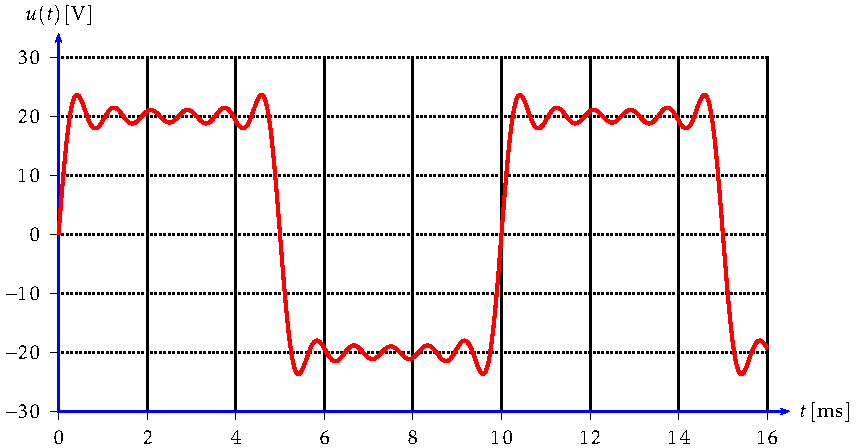
\includegraphics{Imatges/Cap-Fourier-Exemple-Tensio.pdf}
    \end{center}

    La imped\`{a}ncia de la c\`{a}rrega formada per la resist\`{e}ncia $R$ i la
    induct\`{a}ncia $L$, tindr\`{a} un valor $\cmplx{Z}_n$ diferent per a
    cadascuna de les tensions fonamental i harm\`{o}niques presents en la
    tensi\'{o} $u(t)$; els valors de $\cmplx{Z}_n$ per als primes \'{\i}ndex s\'{o}n:

    \begin{alignat*}{3}
        \cmplx{Z}_1 &= R + \ju\, \omega L &&= \SI{10}{\ohm} + \ju\, (200\times \piup\times 50\times 10^{-3})\unit{\ohm} &&=
        \SIpr{32,9691}{1,2626}{\ohm}\\
        \cmplx{Z}_3 &= R + \ju\, 3 \omega L &&= \SI{10}{\ohm} + \ju\, (3\times 200\times \piup\times 50\times 10^{-3})\unit{\ohm} &&=
        \SIpr{94,7768}{1,4651}{\ohm}\\
        \cmplx{Z}_5 &= R + \ju\, 5 \omega L &&= \SI{10}{\ohm} + \ju\, (5\times 200\times \piup\times 50\times 10^{-3})\unit{\ohm} &&=
        \SIpr{157,3976}{1,5072}{\ohm}\\
        \cmplx{Z}_7 &= R + \ju\, 7 \omega L &&= \SI{10}{\ohm} + \ju\, (7\times 200\times \piup\times 50\times 10^{-3})\unit{\ohm} &&=
        \SIpr{220,1387}{1,5254}{\ohm}\\
        \cmplx{Z}_9 &= R + \ju\, 9 \omega L &&= \SI{10}{\ohm} + \ju\, (9\times 200\times \piup\times 50\times 10^{-3})\unit{\ohm} &&=
        \SIpr{282,9201}{1,5354}{\ohm}\\
        \cmplx{Z}_{11} &= R + \ju\, 11 \omega L &&= \SI{10}{\ohm} + \ju\, (11\times 200\times \piup\times 50\times 10^{-3})\unit{\ohm} &&=
        \SIpr{345,7198}{1,5419}{\ohm}
    \end{alignat*}

    L'expansi\'{o} en s\`{e}rie de Fourier del corrent $i(t)$ ser\`{a} an\`{a}loga a la
    de la tensi\'{o} $u(t)$, \'{e}s a dir, tan sols tindr\`{a} funcions sinus
    d'\'{\i}ndex senar. Donat que la c\`{a}rrega \'{e}s inductiva, cadascun dels
    termes del corrent estar\`{a} endarrerit respecte del terme corresponent
    de la tensi\'{o}, en un valor indicat per l'argument de cada imped\`{a}ncia.
    El valor de pic de cada terme del corrent $\hat{I}_n$, s'obt\'{e}
    dividint el valor de pic de cada terme de la tensi\'{o} $\hat{U}_n$ pel
    m\`{o}dul de la imped\`{a}ncia corresponent; els valors de $\hat{I}_n$ per
    als primes \'{\i}ndex s\'{o}n:

    \begin{align*}
        \hat{I}_1 &= \frac{\hat{U}_1}{|\cmplx{Z}_1|} = \frac{80/\piup\unit{V}}{\SI{32,9691}{\ohm}} = \SI{0,7724}{A}
        & \hat{I}_3 &= \frac{\hat{U}_3}{|\cmplx{Z}_3|} =\frac{80/(3\piup)\unit{V}}{\SI{94,7768}{\ohm}} = \SI{0,0896}{A}\\[0.5ex]
        \hat{I}_5 &= \frac{\hat{U}_5}{|\cmplx{Z}_5|} =\frac{80/(5\piup)\unit{V}}{\SI{157,3976}{\ohm}} =\SI{0,0324}{A}
        & \hat{I}_7 &= \frac{\hat{U}_7}{|\cmplx{Z}_7|} =\frac{80/(7\piup)\unit{V}}{\SI{220,1387}{\ohm}} =
        \SI{0,0165}{A}\\[0.5ex]
        \hat{I}_9 &= \frac{\hat{U}_9}{|\cmplx{Z}_9|} =\frac{80/(9\piup)\unit{V}}{\SI{282,9201}{\ohm}} =
        \SI{0,0100}{A} & \hat{I}_{11} &= \frac{\hat{U}_{11}}{|\cmplx{Z}_{11}|} =\frac{80/(11\piup)\unit{V}}
        {\SI{345,7198}{\ohm}} =  \SI{0,0067}{A}
    \end{align*}

    Amb aquests valor calculats, l'expansi\'{o} en s\`{e}rie de Fourier del
    corrent $i(t)$ \'{e}s:

    \[\begin{split}
         i(t) &=  \num{0,7724} \sin(\omega t - \num{1,2626}) +  \num{0,0896} \sin(3 \omega t -
         \num{1,4651}) + \num{0,0324} \sin(5 \omega t - \num{1,5072}) +{}\\
         &+ \num{0,0165} \sin(7 \omega t - \num{1,5254}) + \num{0,0100} \sin(9 \omega t - \num{1,5354})
         + \num{0,0067} \sin(11 \omega t - \num{1,5419}) +\cdots
    \end{split}\]

    A continuaci\'{o} es pot veure la gr\`{a}fica del corrent $i(t)$, que s'obt\'{e}
    utilitzant la seva expansi\'{o} en s\`{e}rie de Fourier, fins a la component
    harm\`{o}nica d'\'{\i}ndex 11:

    \begin{center}
    \centering
      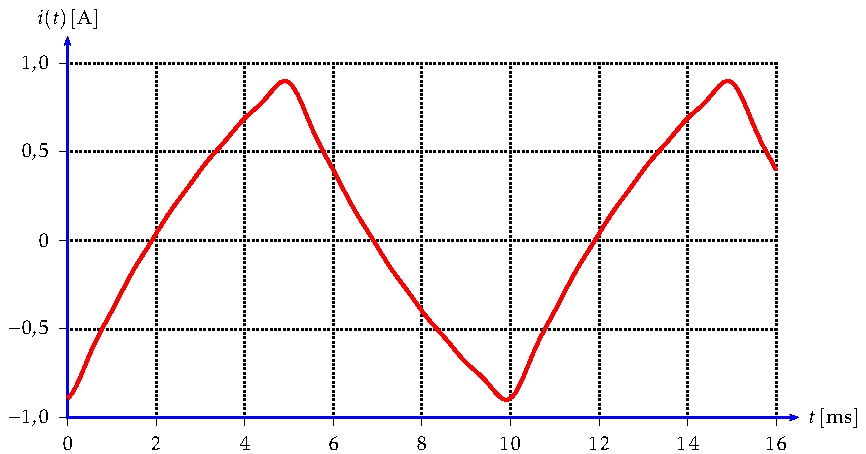
\includegraphics{Imatges/Cap-Fourier-Exemple-Corrent.pdf}
    \end{center}

    Calculem a continuaci\'{o} el valor efica\c{c} $I$ del corrent:
    \[\begin{split}
        I &= \sqrt{\left(\tfrac{\num{0,7724}}{\sqrt{2}}\unit{A}\right)^2 +
            \left(\tfrac{\num{0,0896}}{\sqrt{2}}\unit{A}\right)^2 +
            \left(\tfrac{\num{0,0324}}{\sqrt{2}}\unit{A}\right)^2 +
            \left(\tfrac{\num{0,0165}}{\sqrt{2}}\unit{A}\right)^2 +
            \left(\tfrac{\num{0,0100}}{\sqrt{2}}\unit{A}\right)^2 +
            \left(\tfrac{\num{0,0067}}{\sqrt{2}}\unit{A}\right)^2 + \cdots}
            \,\approx \\[1ex]
            &\approx \SI{0,5505}{A}
    \end{split}\]

    Finalment, la pot\`{e}ncia $P$ dissipada en la resist\`{e}ncia ser\`{a}:
    \[
        P = R I^2 \approx \SI{10}{\ohm} \times (\SI{0,5505}{A})^2 =
        \SI{3,03}{W}
    \]

    Aquest valor tamb\'{e} es pot calcular a partir de l'equaci\'{o}
    \eqref{eq:pot_fu}. La pot\`{e}ncia aix\'{\i} calculada, correspon a la
    pot\`{e}ncia activa cedida per la font de tensi\'{o}, i donat que la
    resist\`{e}ncia $R$ \'{e}s l'\'{u}nic component del circuit que en consumeix,
    aquest m\`{e}tode ens proporcionar\`{a} el mateix resultat; utilitzant les
    expansions en s\`{e}rie de Fourier de la tensi\'{o} $u(t)$ i del corrent
    $i(t)$, fins a la component harm\`{o}nica d'\'{\i}ndex 11, tenim:

    \[\begin{split}
        P &\approx U_1 I_1 \cos\varphi_1 +  U_3 I_3 \cos\varphi_3 +
         U_5 I_5 \cos\varphi_5 + U_7 I_7 \cos\varphi_7 +
         U_9 I_9 \cos\varphi_9 + U_{11} I_{11} \cos\varphi_{11} = {}\\[0.7ex]
        &= \frac{80}{\piup\times\sqrt{2}}\unit{V} \times
        \frac{\num{0,7724}}{\sqrt{2}}\unit{A} \times \cos \num{1,2626} +
        \frac{80}{3\times\piup\times\sqrt{2}}\unit{V} \times
        \frac{\num{0,0896}}{\sqrt{2}}\unit{A} \times \cos \num{1,4651} + {} \\[0.7ex]
        &+ \frac{80}{5\times\piup\times\sqrt{2}}\unit{V} \times
        \frac{\num{0,0324}}{\sqrt{2}}\unit{A} \times \cos \num{1,5072} +
        \frac{80}{7\times\piup\times\sqrt{2}}\unit{V} \times
        \frac{\num{0,0165}}{\sqrt{2}}\unit{A} \times \cos \num{1,5254} + {}\\[0.7ex]
        &+ \frac{80}{9\times\piup\times\sqrt{2}}\unit{V} \times
        \frac{\num{0,0100}}{\sqrt{2}}\unit{A} \times \cos \num{1,5354} +
        \frac{80}{11\times\piup\times\sqrt{2}}\unit{V} \times
        \frac{\num{0,0067}}{\sqrt{2}}\unit{A} \times \cos \num{1,5419}= {}\\[0.7ex]
        &= \SI{3,03}{W}
    \end{split}\]

    En la resoluci\'{o} d'aquest exemple, hem emprat tan sols els sis
    primers termes de las s\`{e}ries de Fourier de la tensi\'{o} i del corrent;
    no obstant, el valor  obtingut de la pot\`{e}ncia ha de ser prou prec\'{\i}s, ja que
    els valors de pic dels termes de la s\`{e}rie del corrent, disminueixen de
    valor r\`{a}pidament.

    Refarem a continuaci\'{o} els c\`{a}lculs utilitzant m\'{e}s termes, amb l'ajut
    del programa
    \textit{Mathematica}${}^\circledR$.
    \index{Mathematica@\textit{Mathematica}${}^\circledR$}
    Definim en primer lloc el valor de pic de cada
     terme de la tensi\'{o} i el valor del m\`{o}dul de la imped\`{a}ncia corresponent,
    calculem a continuaci\'{o} els 100 primers termes del corrent de pic, i
    per acabar calculem el valor efica\c{c} del corrent i la pot\`{e}ncia:

    \begin{alltt}
    \bfseries In[1]:= u[n_] = 80 / (Pi (2n-1));\\
     In[2]:= z[n_] = Abs[10 + I (2n-1) 200 Pi 50 10^-3];\\
     In[3]:= i = Table[u[n], \{n, 1, 100\}] / Table[z[n], \{n, 1, 100\}];\\
     In[4]:= Irms = Sqrt[Apply[Plus, (i/Sqrt[2])^2]] // N\\
    Out[4]:= 0.550511\\
     In[5]:= P = 10 Irms^2\\
    Out[5]:= 3.03063
    \end{alltt}

    Tamb\'{e} podem fer aquests c\`{a}lculs amb el programa
    MATLAB${}^\circledR$, tal com es veu a continuaci\'{o}:
    \index{MATLAB@\textit{MATLAB}${}^\circledR$}
    \begin{alltt}
    \bfseries>> u = 80./(pi*(2*[1:1:100]-1));\\
    >> z = abs(10 + i*(2*[1:1:100]-1)*200*pi*50*1e-3);\\
    >> i = u./z;\\
    >> Irms = sqrt(sum((i./sqrt(2)).^2))\\
    Irms =\\
        0.5505\\
    >> P = 10*Irms^2\\
    P =\\
        3.0306
    \end{alltt}

     Com es pot observar, el valor de la pot\`{e}ncia obtingut amb qualsevol dels dos
     programes,
     coincideix d'una manera prou aproximada, amb el valor calculat a m\`{a}
    anteriorment.
\end{exemple}
